\subsection{What is a Karp-reduction?}
\label{karpwhat}

When we say that a Karp-reduction $Left \prec Right$ exists, it means all of these things:

(Where $Left$ and $Right$ are both some decision problems. Traditionally we would use letters, like $X \prec Y$, or the name of the actual problems, but I replaced them with $Left$, meaning left side and $Right$ right side, it makes the following stuff more readable.)

\begin{itemize}
    \item $Left$ can be solved using $Right$.
    \item The hardness of $Left$ cannot be more, than the hardness of $Right$, since $Left$ can be solved using $Right$.
    \item The way we can solve $Left$ with using $Right$ is very specific:
    \begin{itemize}
        \item We take the input meant to be given to $Left$.
        \item We run in through a \textbf{polynomial time transformation}, which we note by function $f$.
        \item Then we give the transformed input to $Right$.
        \item Then whatever $Right$ outputs, we must respond with the same thing. (This can be tricky to achieve!)
    \end{itemize}
    \item The polynomial-time transformation is usually noted by $f$. It must be created in a way, so that the YES / NO answers are the same: for any input $Left$ answers with a $YES$, the transformed input must result in a $YES$ answer from $Right$ as well, and same for the answer $NO$.
\end{itemize}

You can think about it like this:

\begin{center}
    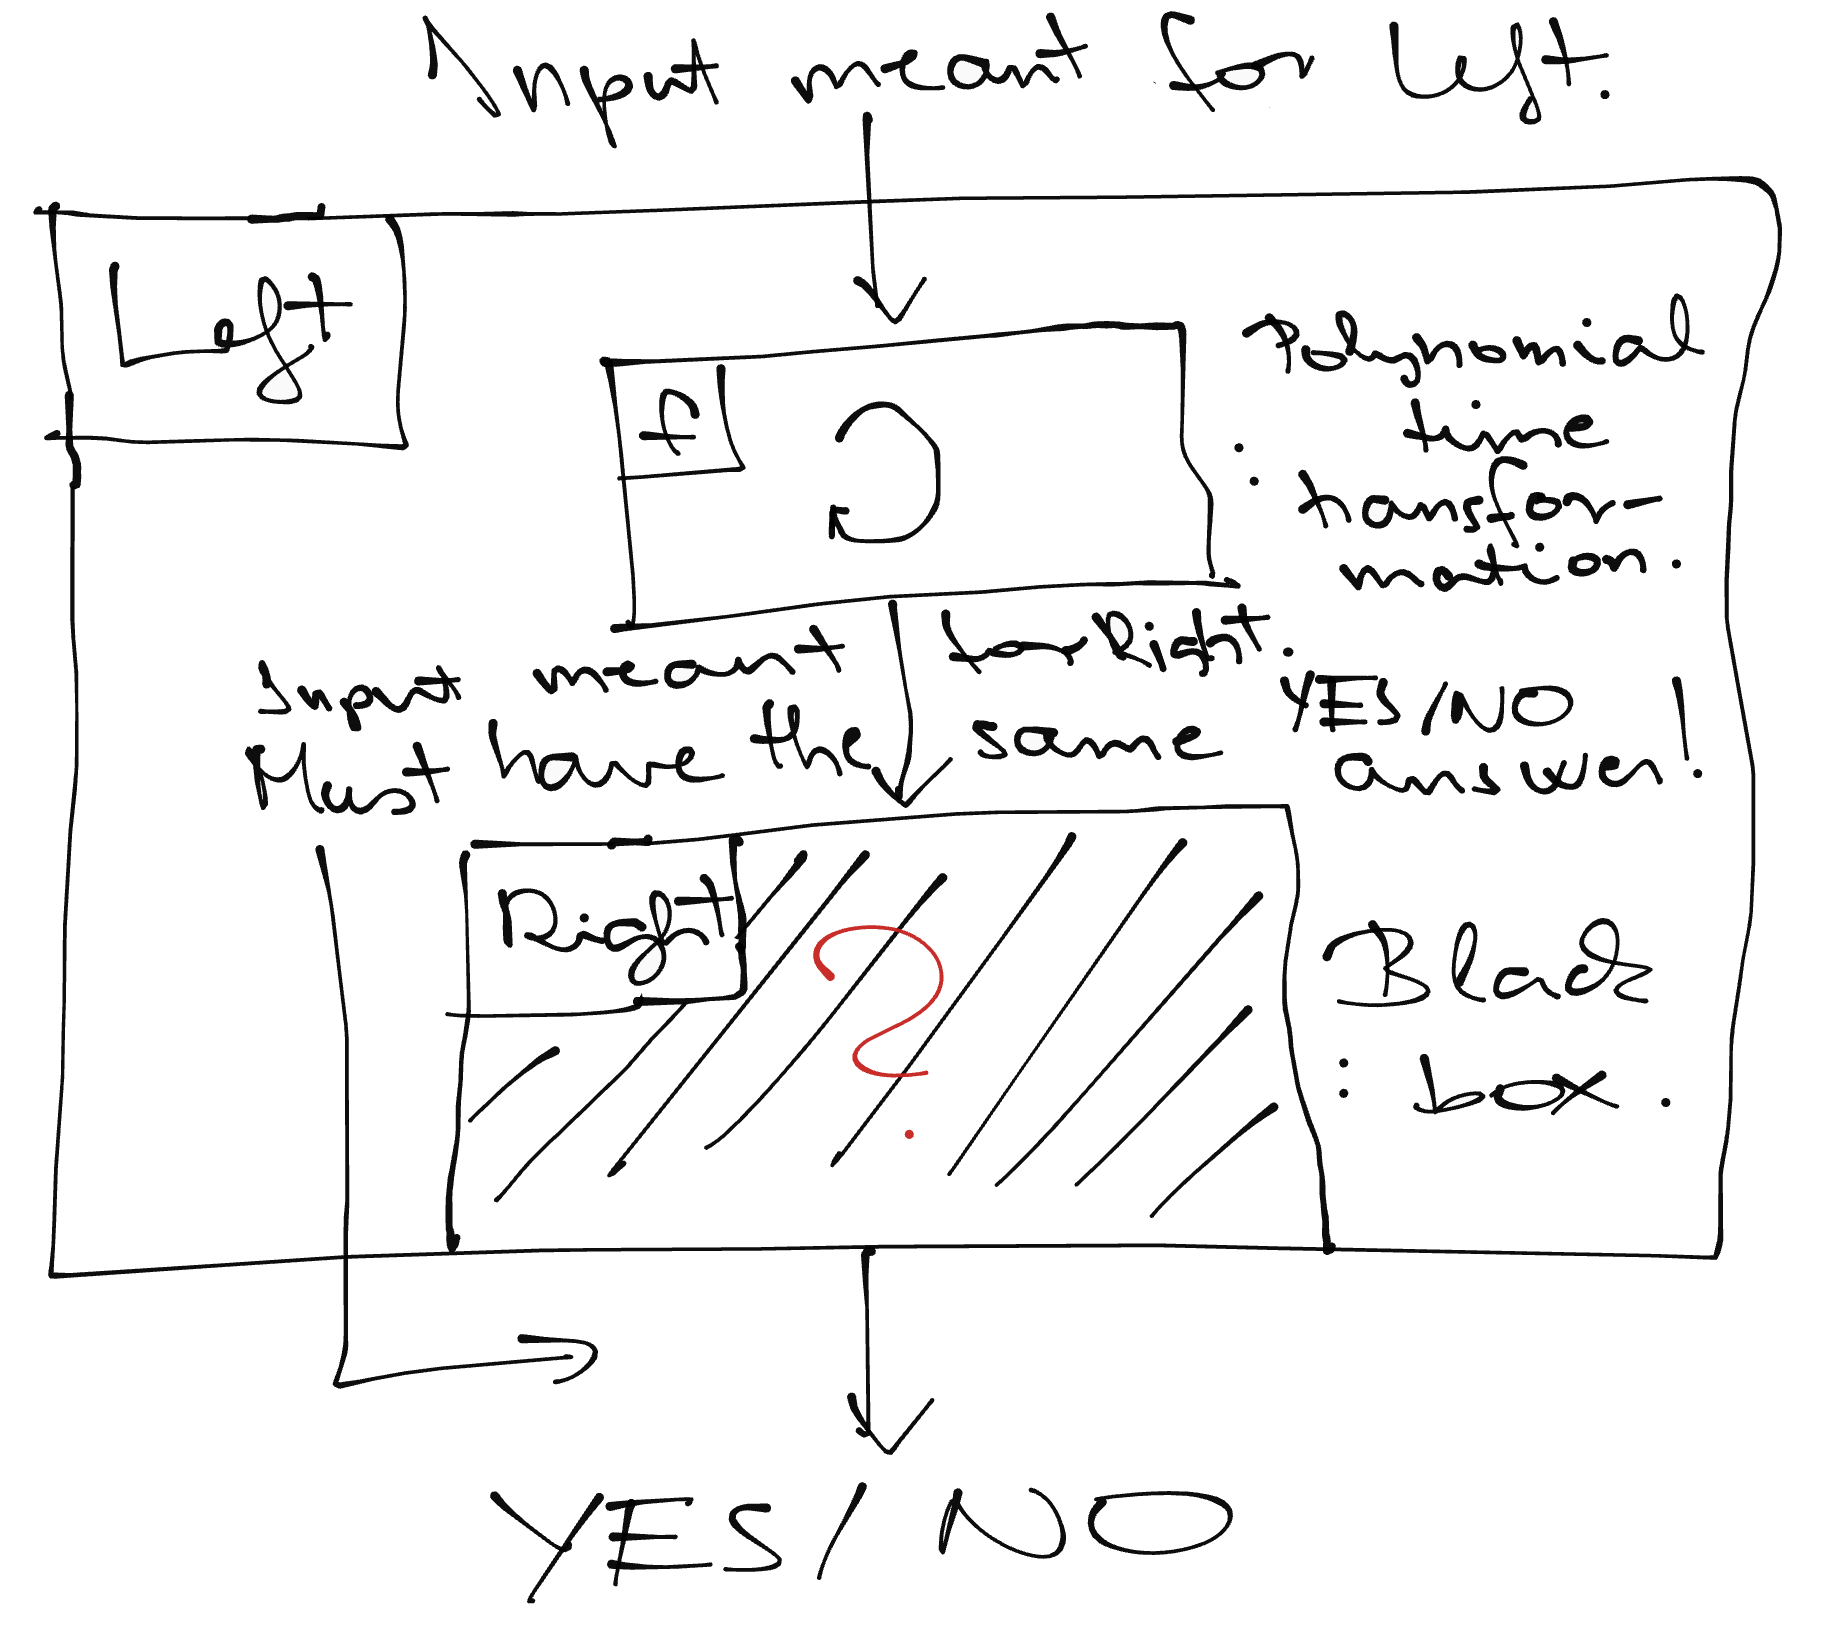
\includegraphics[width=0.8\linewidth]{08/01/karp_reduction.png}
\end{center}

Notice, how $Right$ is attached to the bottom of $Left$, this is meant to show, that we cannot modify that answer, we must return it immediately. (By the way, other polynomial-time reductions exist, which allow you to run the $Right$ algorithm multiple times, or modify the output, but we do not study these.)

It can be difficult to remember the order of these (which one is used to solve which one?), for that I suggest remembering the phrase: ''When there is nothing (to solve) $Left$, one must do the (algorithm to solve the) $Right$ thing!''

The reason why they invented polynomial-time reductions, like the Karp-reduction is because groups of researchers have been struggling for a very long time to come up with efficient solutions for a number of very important problems (these are the $NP$-complete problems we are studying). They have started to notice, that these problems did not differ from one another by that much, in fact, if someone came up with a fast solution to one of these problems, the others could create a solution for theirs by running a fast tranformation of their input and then using the solution for the other. Essentially, we cannot (yet? or not at all?) solve these problems, but we are prepared for a solution to one of them pop up, since we have done all the work to solve everything else from that. We are just waiting for that one solution...

This video talks about this, I highly recommend checking it out: \href{https://youtu.be/YX40hbAHx3s}{P vs. NP and the Computational Complexity Zoo from hackerdashery}.

Whenever you are given a task to give a Karp-reduction between two problems, I see a lot of confusion on what the task is asking for. I would like to use an example and answer common questions on it: let's say you need to give a Karp-reduction $s-t-HAMPATH \prec HAM$.

\begin{itemize}
    \item Which one is being used to solve which one?
    
    $\rightarrow$ The left is solved using the right one, so in this case $s-t-HAMPATH$ is solved using an imaginary preexisting solution to $HAM$.
    \item Did someone solve $HAM$ but struggles to solve $s-t-HAMPATH$? These are almost the same, we should just look at the code and fix it up!
    
    $\rightarrow$ We do not know anything about the solution to $HAM$, we cannot look at the code. This is because nobody actually solved $HAM$ yet. We can imagine if someone solved $HAM$, then we could probably modify the code and solve $s-t-HAMPATH$ too with it, but without knowing what the solution is, all we can do is treat it as a blackbox.
    
    \item Why can't we change the result? For example, what if we wanted to return $YES$ any time $Right$ says $NO$ and vice versa? Why can't we run the algorithm for $Right$ more than once, for differently transformed inputs and collect and make sense of the result?
     
    $\rightarrow$ This is specific to this type of polynomial-time reduction. Other's exist for which the rules are different, but we don't study those. I've talked about this on the practice sessions: limitations like this usually exist, because they make it easier to give proofs. The less stuff can happen, the easier it is to argue. Then, in practice we usually use a less-rule-limited version of stuff, with proofs that the less-rule-limited version can't actually do more than the rule-limited version.
    
    \item How do we create the Karp-reduction?
    
    $\rightarrow$ You give the $f$ polynomial time transformation:
    \begin{itemize}
        \item First, you explain what the inputs and outputs are for $HAM$ and $s-t-HAMPATH$.
        \begin{itemize}
            \item $HAM$'s input is an undirected graph, for which it checks whether it contains a Hamiltonian cycle. (If it does, it returns $YES$, if it does not, it returns $NO$.)
            \item $s-t-HAMPATH$'s input is an undirected graph, and two vertices of that graph, one is noted by $s$, the other is noted by $t$. It checks if there exists a Hamiltonian path between vertices $s$ and $t$ in the graph (returns $YES$ if exists, returns $NO$, if does not).
            \item (Hamiltonian \textit{something} means that the \textit{something} contains all vertices of the graph.)
        \end{itemize}
        \item Then, you explain what the input transformation is.
        \begin{itemize}
            \item It is very important here, that it is very likely not just a copy and paste of whatever input matches and then fill in the rest!
            \item  So in this case, we will have to modify the $G$ graph, since just giving it straight to a solver that's trying to find a Hamiltonian cycle in it, while we only need a Hamiltonian path is not going to work.
            \item If the graph has a Hamiltonian cycle, then it also has a Hamiltonian path, however that path might not be so that $s$ and $t$ are neighbours on it (so the $s-t-$Hamiltonian path does not exist, that part of the path does not contain all vertices), and it could be that the graph does not have a Hamiltonian cycle, but it does have the $s-t$-Hamiltonian path (a single $s-t$ edge is missing to complete the cycle).
            \item In this case, the transformation is the following: add one more vertex to the graph, note it with $v$, and connect it to the vertices $s$ and $t$.
        \end{itemize}
        \item Then, you explain why any input for $s-t-Hampath$ that is a $YES$ answer, if we transform the input in the specified way, the answer will be $YES$ for $HAM$ as well.
        \begin{itemize}
            \item If there was an $s-t$-Hamiltonian path in $G$, then the edges of the Hamiltonian cycle in the transformed $G'$ graph will be the edges of the $s-t$-Hamiltonian path + the $s-v$ and $v-t$ edges we added.
            \item This contains all vertices from $G$, plus the one additional vertex $v$ as well, making it a Hamiltonian cycle.
        \end{itemize}
        \item Then, you explain the same for he $NO$ answers (usually this will be an indirect proof):
        \begin{itemize}
            \item If there is no $s-t$-Hamiltonian path in $G$, then there cannot be a Hamiltonian cycle in $G'$. Why? Let's argue using indirect proof: let's indirectly assume that there is no $s-t$-Hamiltonian path in $G$, but there still exists a Hamiltonian cycle in $G'$. Then, if we remove the vertex $v$ from that cycle, we will be left with a path that contains all other vertices of the $G'$, so all original vertices of $G$, plus the endpoints of that path will be $s$ and $t$, since $v$ was only connected to those two, so they must also be neighbours on the Hamiltonian cycle. This is a contradiction, since we assumed no $s-t$-Hamiltonian path exists, so this proves our original statement.
        \end{itemize}
        \item Finally, you explain why the transformation can be done in polynomial time (don't forget this step, if the transformation is too slow, then we can't use it in a fast solution for $s-t-HAMPATH$).
        \begin{itemize}
            \item Graphs are given by their adjacency matrices.
            \item To add one more vertex to the graph, we append one row and one column to this matrix (copy the entire thing into a matrix that has one extra column and row).
            \item We add $1$'s to this row at the indexes corresponding to $s$ and $t$. If the adjacency matrix is of size $n^2$, then this can be done in $O(n^2)$ time, which is linear relative to $n^2$.
        \end{itemize}
    \end{itemize}
\end{itemize}

I also like to imagine Karp-reduction with the following fictive code:

\begin{minted}[linenos]{c++}
#include <vector>
using namespace std;
using adj = vector<vector<int>>; // Declare type for adjacency matrix.

// Karp came up with this idea...
bool s_t_hampath_solver(adj G, int s, int t) {
    vector<vector<int>> G_prime = f(G, s, t);
    return ham_solver(G_prime);
}

// ..and asked you to implement this part:
vector<vector<int>> f(adj G, int s, int t) { // Totally polynomial!
    int size = G.size();
    vector<vector<int>> G_prime(size+1, size+1);
    for(int i=0; i<size; ++i) {
        for(int j=0; j<size; ++j) {
            G_prime[i][j] = G[i][j];
        }
    }
    int v = size; // Indexing starts with 0.
    G_prime[v][s] = 1;
    G_prime[v][t] = 1;
    G_prime[s][v] = 1;
    G_prime[s][t] = 1;
    return G_prime;
}

bool ham_solver(adj G) {
    // TODO
}
\end{minted}